\subsection{Comparison of Prediction Methods}

EG01-EG23, EG01-EG24, EG01-EG29, and EG01-EG30 transition scenarios
are set up in \Cyclus using \deploy. 
To determine the most effective \deploy prediction methods, a
comparison of each prediction method for each 
transition scenarios is conducted for constant power 
and linearly increasing power demand. 
Similar to the basic transition scenarios, these transition scenario 
simulations begin with an initial fleet of \glspl{LWR} and after 
80 years, the simulation progressively decommissions the \glspl{LWR}, 
and \deploy deploys \glspl{FR} to meet the unmet power demand. 
Figure \ref{fig:eg2329}
show the set up of facilities and mass flows for 
EG1-23 and EG1-29 in \Cyclus. 
In EG1-23 and EG1-29, only plutonium is recycled from \gls{LWR}
spent fuel to produce \gls{FR} fuel. 
EG1-24 and EG1-30 are similar to EG1-23 and EG1-29 respectively,
with exception that all transuranic elements are recycled.  

\begin{figure}[]
	\centering
	\begin{subfigure}[t]{\textwidth}
		\centering
		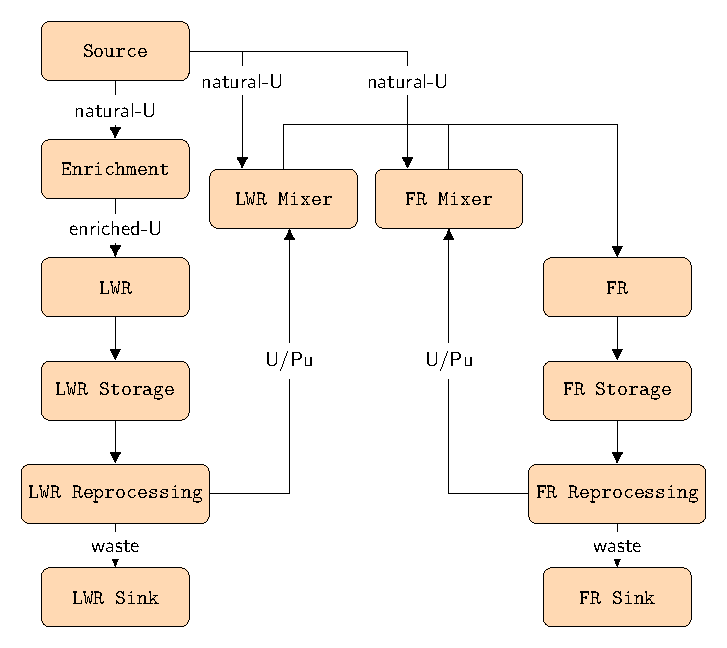
\includegraphics[width=0.55\linewidth]{23flow.pdf} 
		\caption{EG01-EG23.}
		\label{fig:23flow}
	\end{subfigure}
	\vspace{1cm}
	\begin{subfigure}[t]{\textwidth}
		\centering
		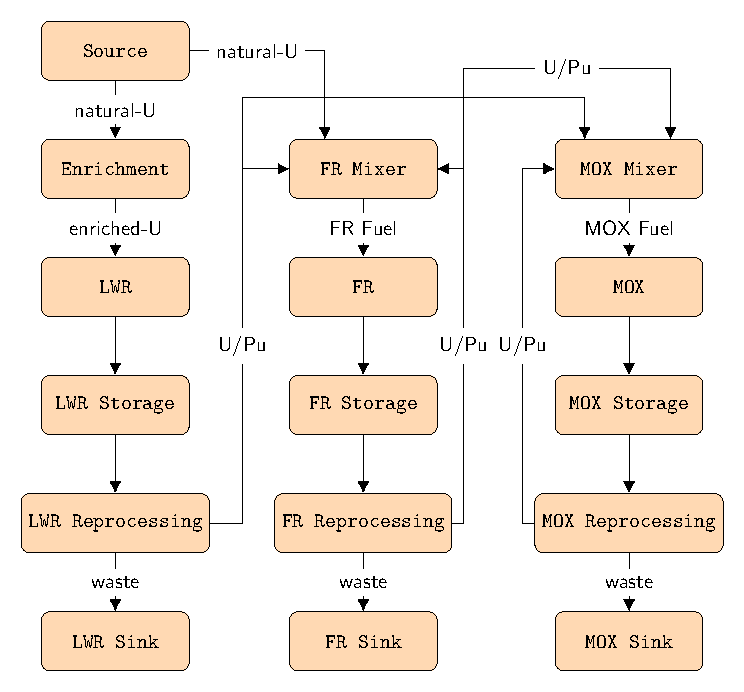
\includegraphics[width=0.55\linewidth]{29flow.pdf} 
		\caption{EG01-EG29.}
		\label{fig:29flow}
	\end{subfigure}
	\hfill
	\caption{Diagrams with facilities and mass flow of the scenarios EG01-EG23 and EG01-EG24.}
	\label{fig:eg2329}
\end{figure}

Figure \ref{fig:eg23under} shows the time steps in which there is undersupply 
of each commodity for a constant power EG01-23 scenario for varying 
prediction methods.
The size of the points are normalized to the largest undersupply
value, therefore, the bigger the point, the larger the undersupply. 
The poly and fft methods perform the best, with poly performing slightly 
better at minimizing under supply of power.
A similar plot was created for a constant power EG1-29 scenario, and 
it was found that poly also performed best for minimizing under supply 
of power.  

Figure \ref{fig:eg24under} shows the time steps in which there is undersupply 
of each commodity for a linearly increasing power EG01-24 scenario for varying 
prediction methods.
The size of the points are normalized to the largest undersupply
value, therefore, the bigger the point, the larger the undersupply. 
The fft method performs the best at minimizing under supply of all 
commodities.
A similar plot was created for a constant power EG1-30 scenario, and 
it was found that poly and fft performed best for minimizing under supply 
of all commodities.  

\begin{figure}[]
	\centering
	\begin{subfigure}[t]{1.2\textwidth}
		\centering
		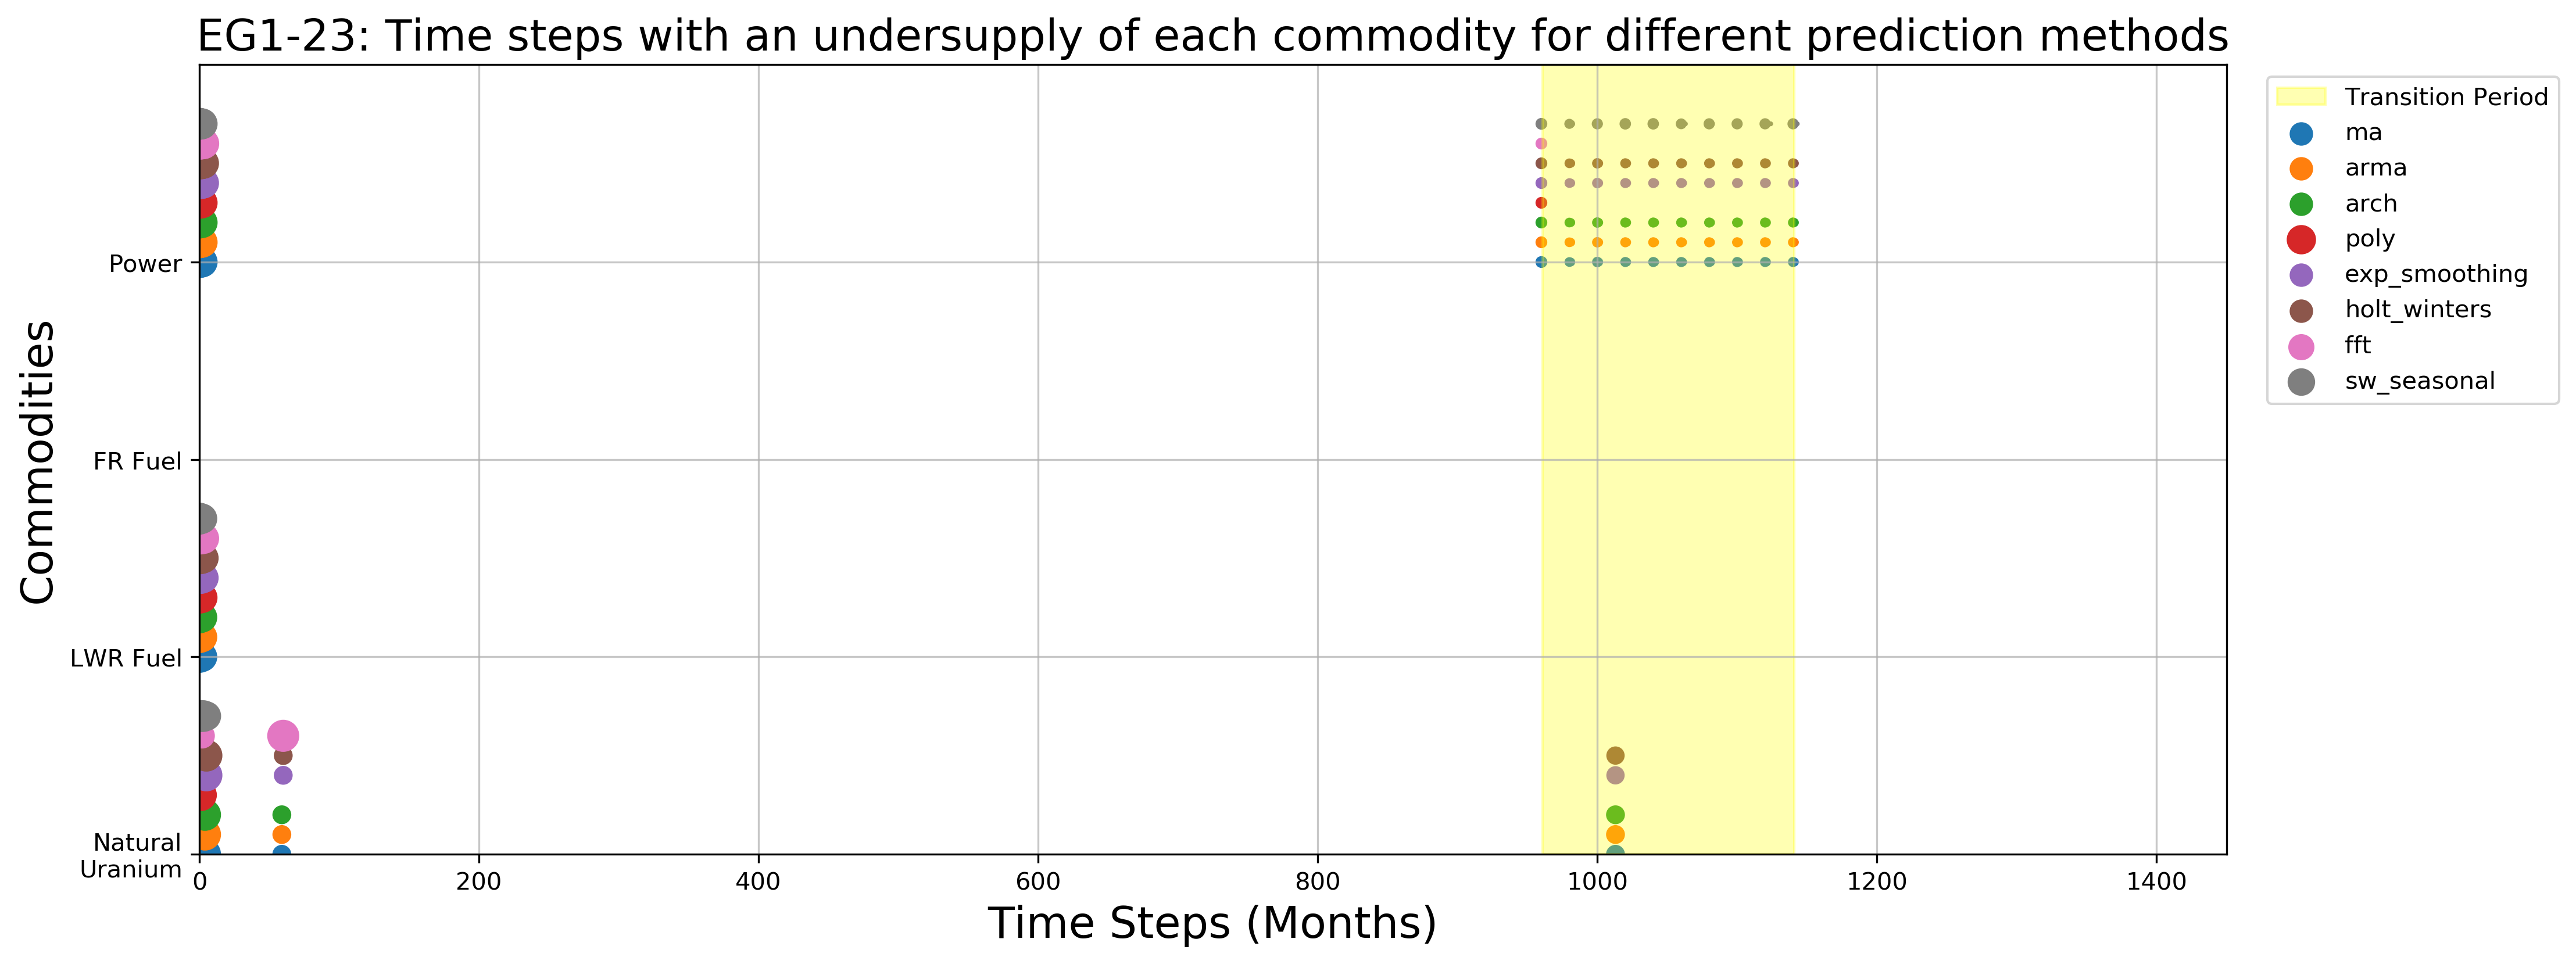
\includegraphics[width=\linewidth]{eg23-undersupply.png} 
		\caption{Under Supply}
		\label{fig:23undersupply}
	\end{subfigure}
	\vspace{1cm}
	\begin{subfigure}[t]{1.2\textwidth}
		\centering
		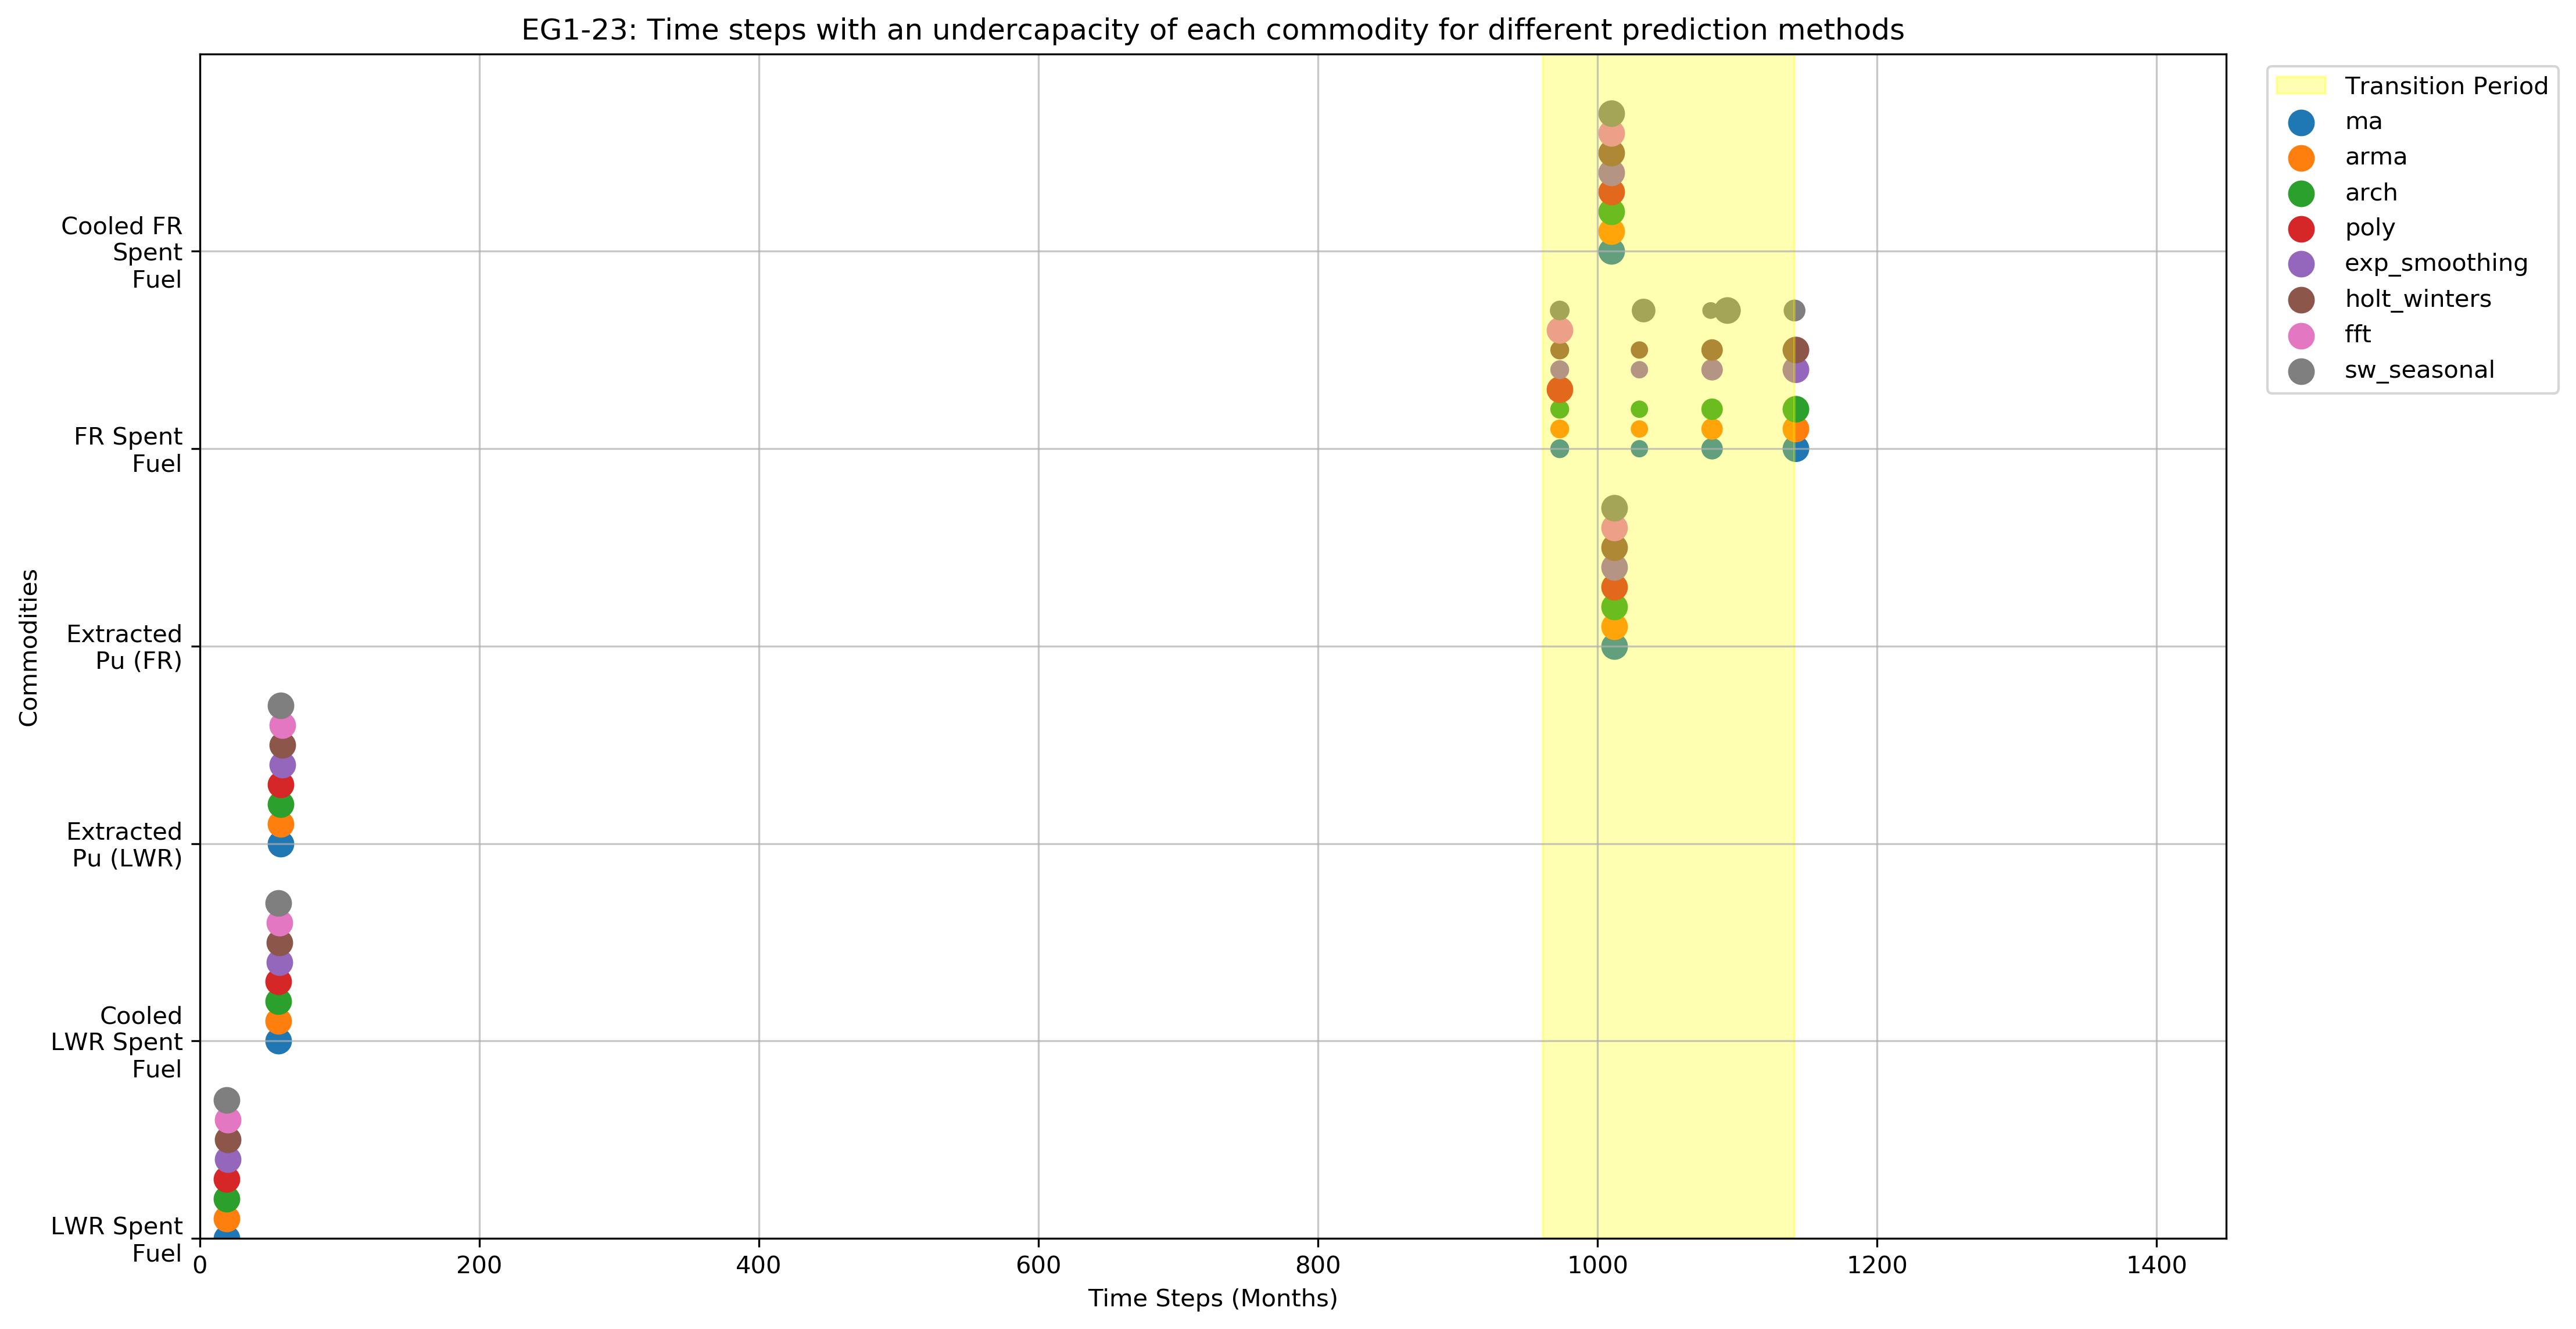
\includegraphics[width=\linewidth]{eg23-undercapacity.png} 
		\caption{Under Capacity}
		\label{fig:23undercapacity}
	\end{subfigure}
	\hfill
	\caption{Comparison of undersupply}
	\label{fig:eg23under}
\end{figure}

\begin{figure}[]
	\centering
	\begin{subfigure}[t]{1.2\textwidth}
		\centering
		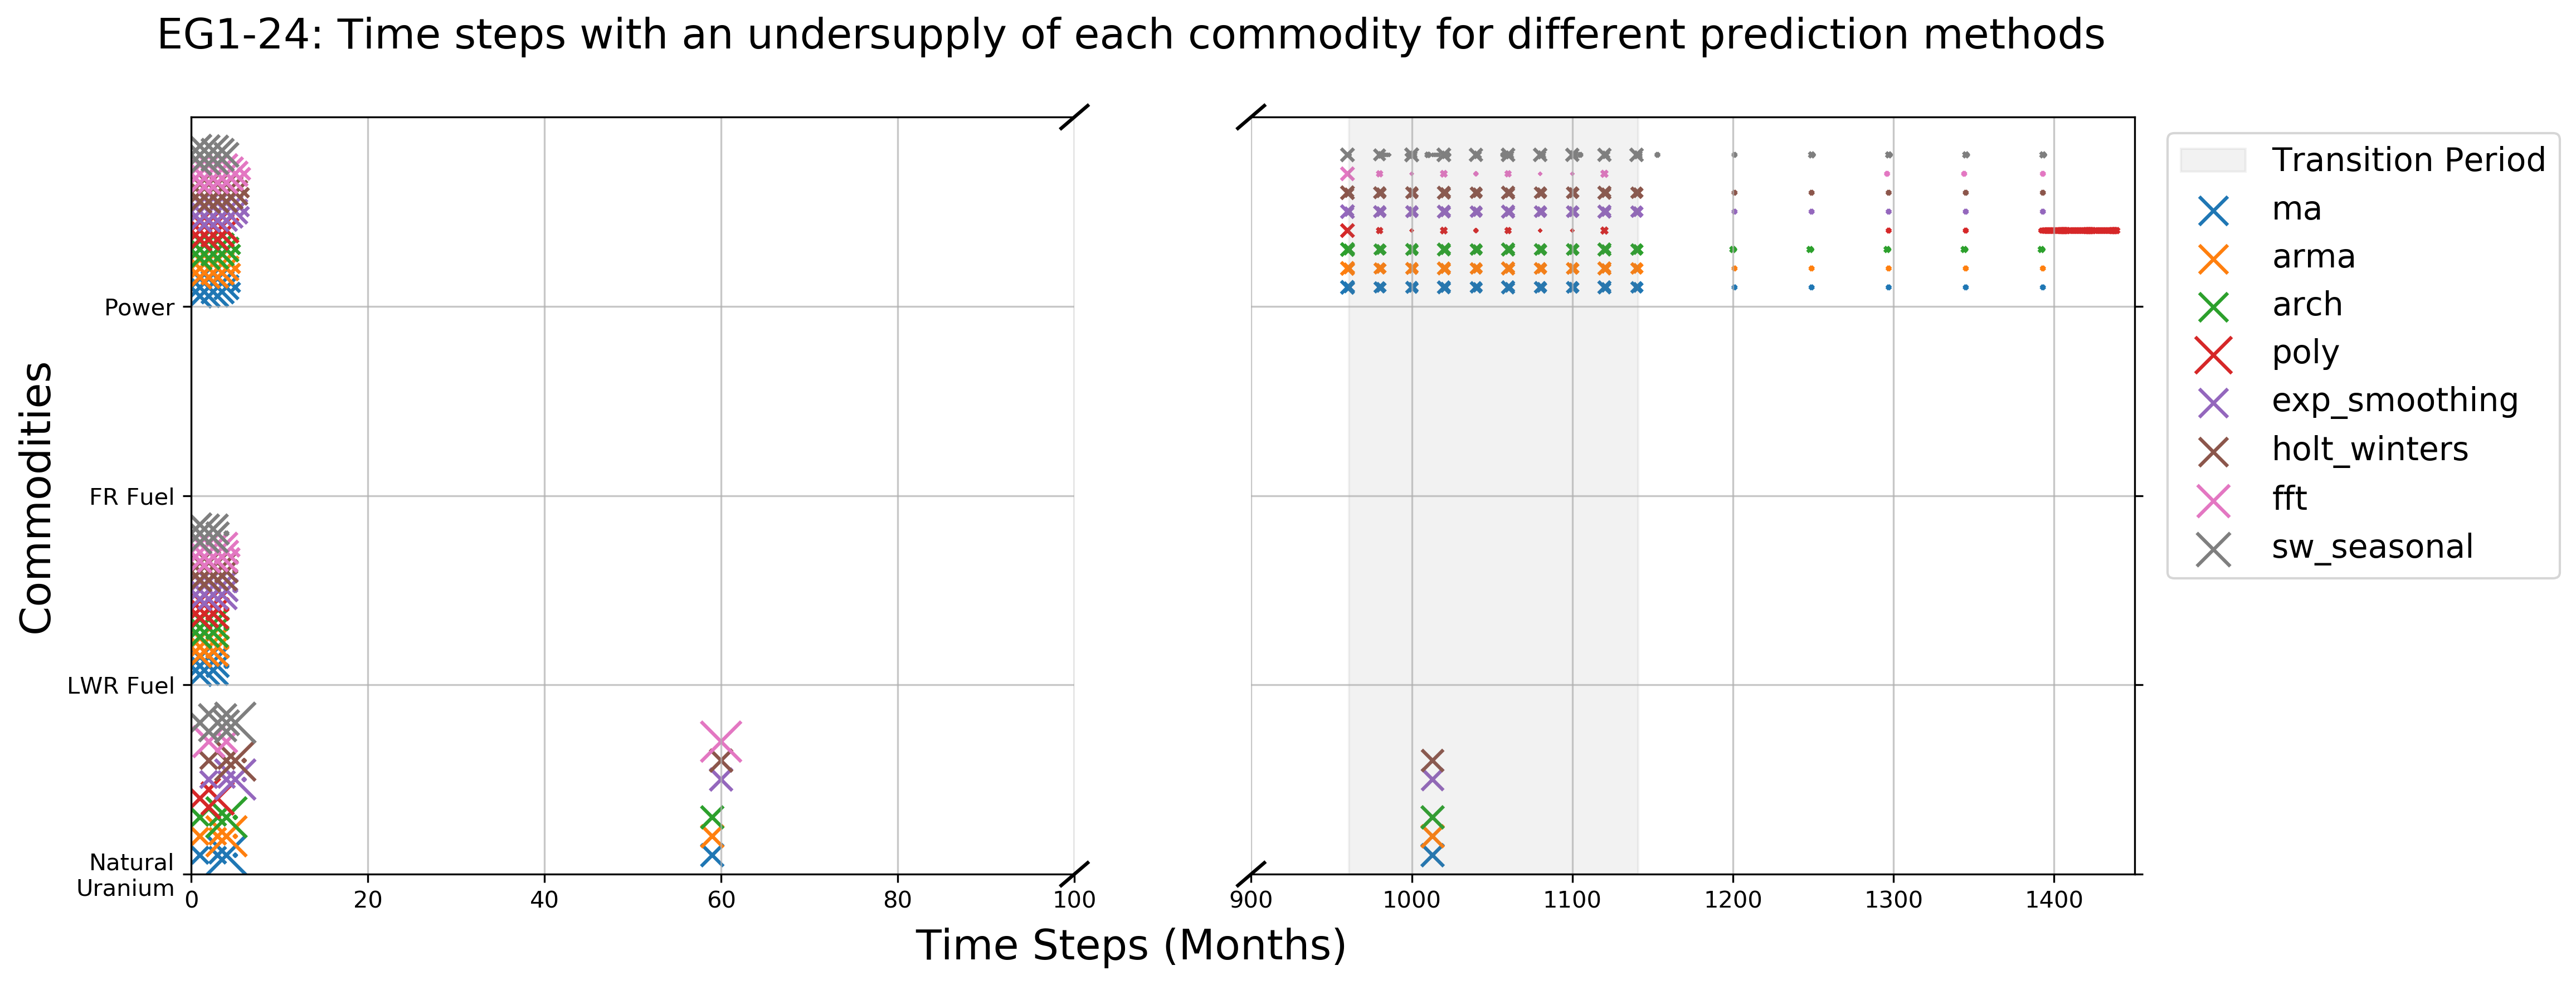
\includegraphics[width=\linewidth]{eg24-undersupply.png} 
		\caption{Under Supply}
		\label{fig:24undersupply}
	\end{subfigure}
	\vspace{1cm}
	\begin{subfigure}[t]{1.2\textwidth}
		\centering
		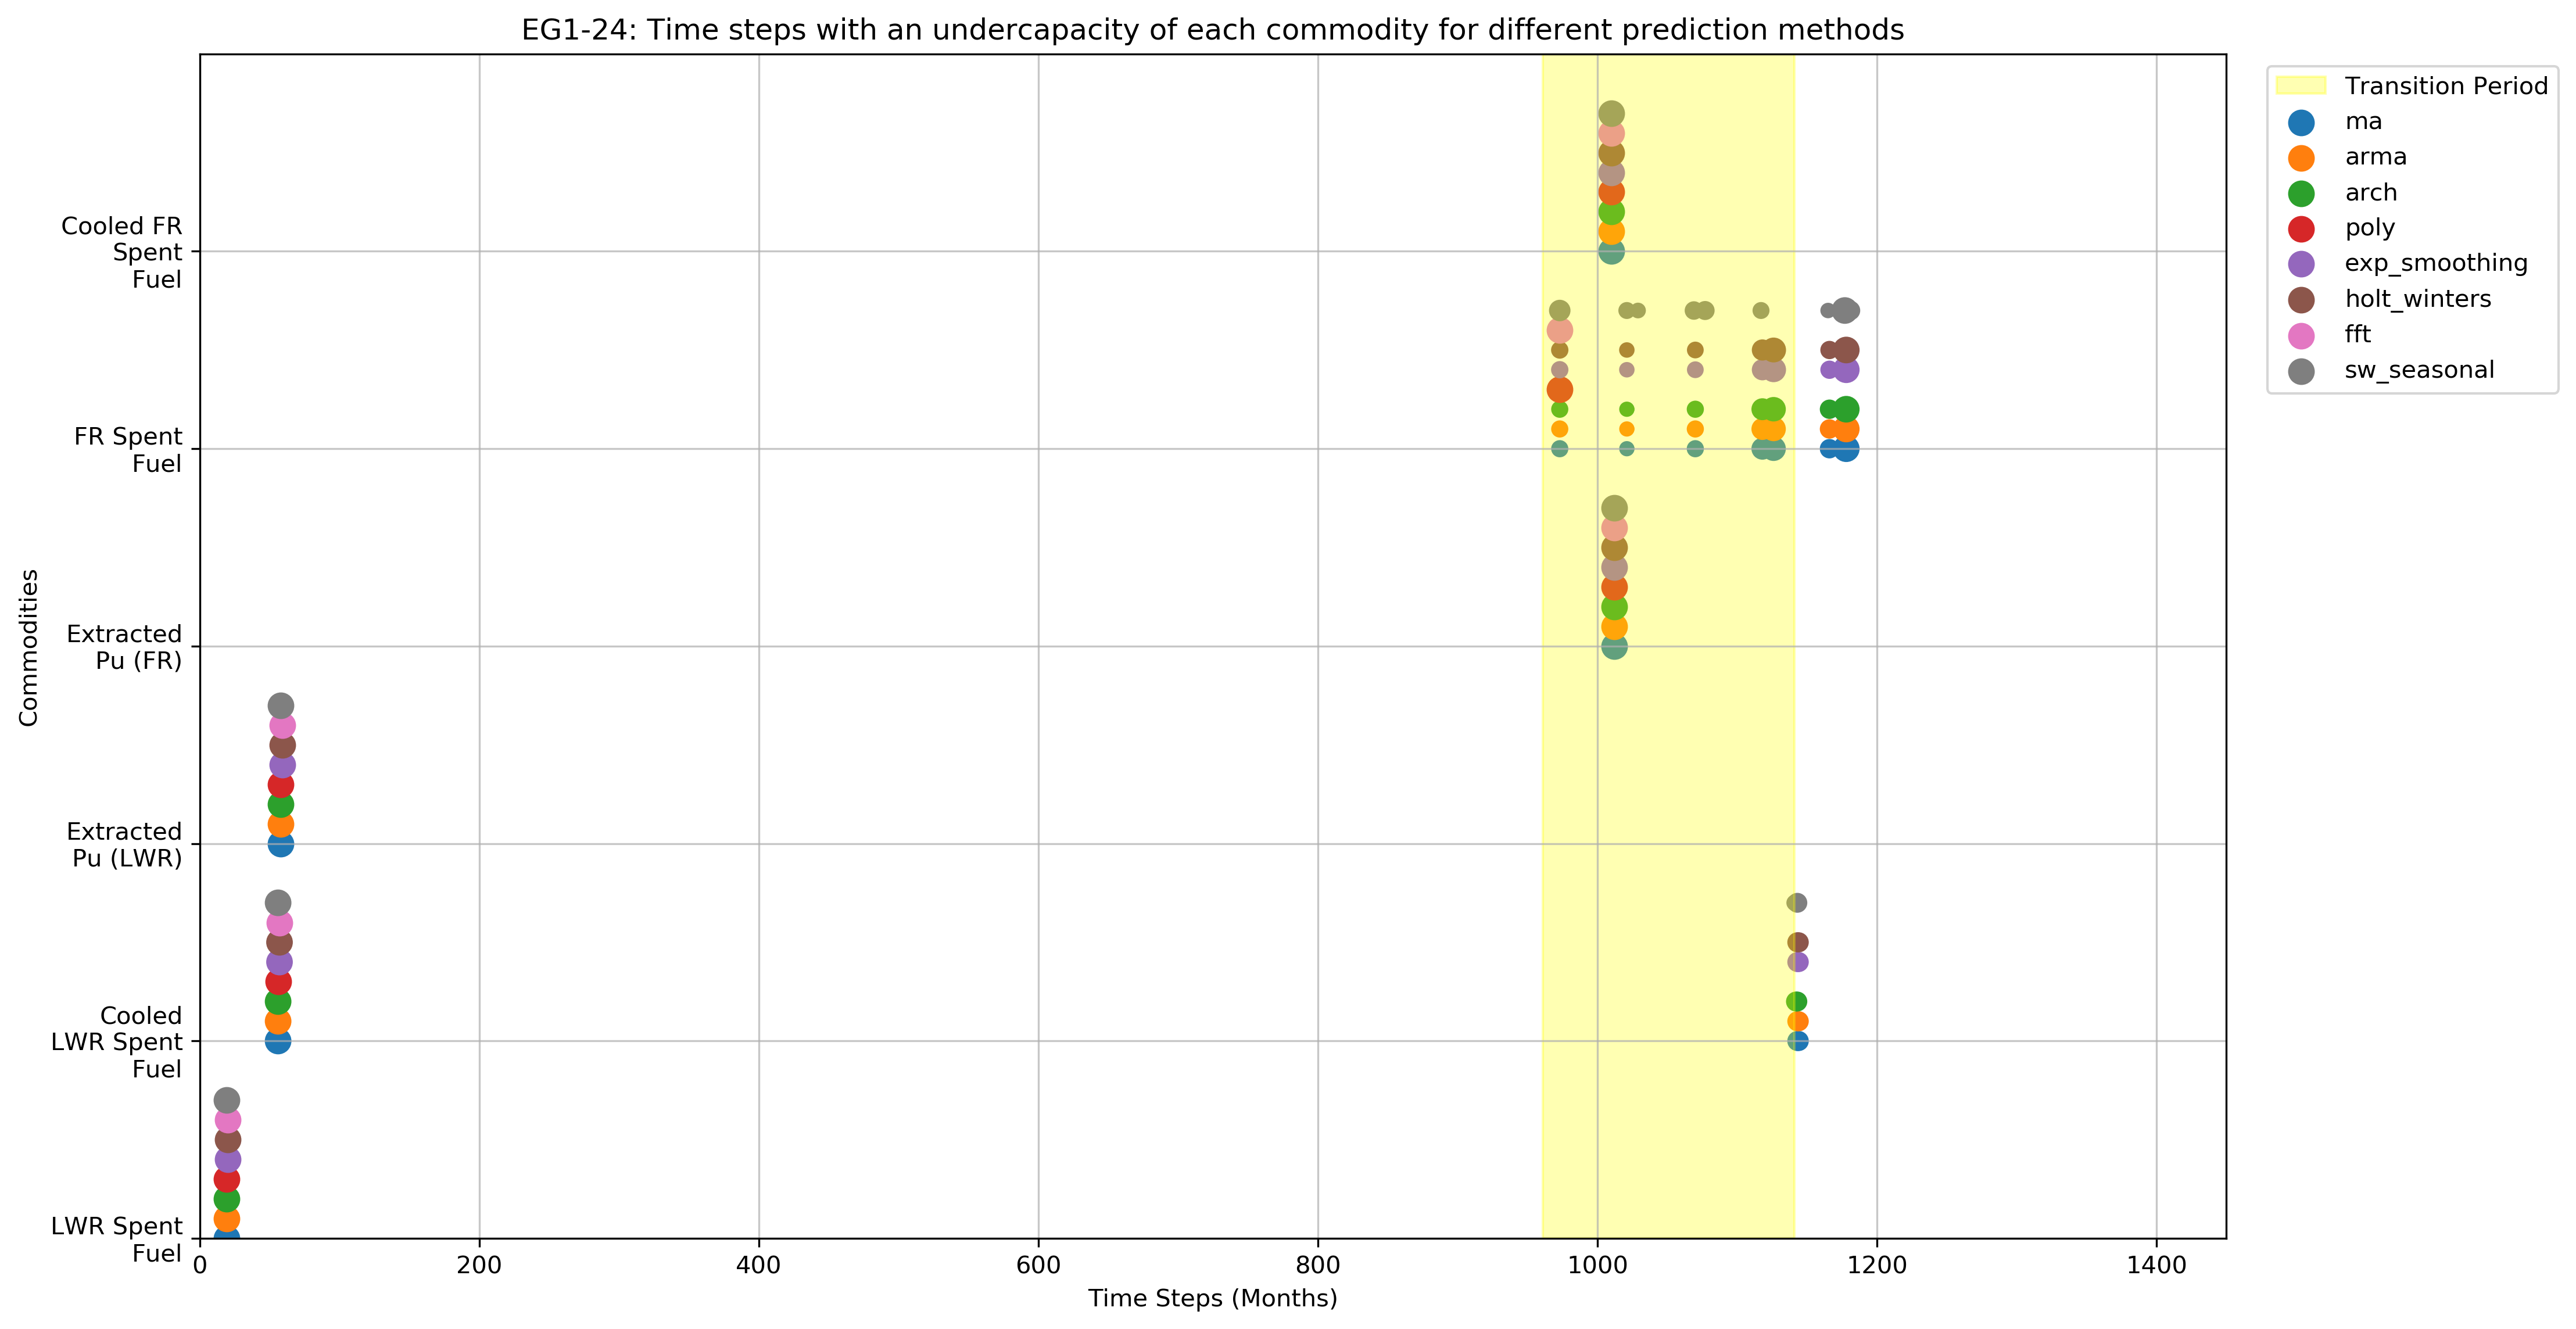
\includegraphics[width=\linewidth]{eg24-undercapacity.png} 
		\caption{Under Capacity}
		\label{fig:24undercapacity}
	\end{subfigure}
	\hfill
	\caption{Comparison of undersupply}
	\label{fig:eg24under}
\end{figure}

Table \ref{tab:all-power} shows the number of time steps with power 
undersupply for constant power EG01-EG23 and EG01-29, 
linearly increasing power EG01-24 and EG01-30 transition scenarios. 
The ideal transition scenario eliminates power undersupply and 
minimizes power oversupply. 

\begin{table}[]
	\centering
        \caption{Undersupply and oversupply of power with the different 
        algorithms used to drive EG01-EG23,24,29,30.}
		\label{tab:all-power}
		\footnotesize
        \begin{tabularx}{\textwidth}{l|RRRR}
		\hline
		& \multicolumn{3}{|c}{\textbf{Power Undersupplied Time Steps}} \\ \hline
		Algorithm & EG01-EG23 Constant Power  & 
		EG01-EG24 Linearly Increasing Power   & EG01-EG29 Constant Power & 
		EG01-EG30 Linearly Increasing Power \\ \hline
		MA     		    & 26 	& 36  &  15  & 24 \\ 
		ARMA     	    & 26 	& 36  &  15  & 24\\ 
		ARCH     	    &  26 	& 36  &  15  & 21\\ 
		POLY      		&  6 	& 65  &  4 &  9\\ 
		EXP\_SMOOTHING 	& 27 	& 37  & 16 & 25\\ 
		HOLT-WINTERS  	& 27 	& 37  & 16 & 25\\ 
		FFT       		& 8 	& 20  & 5 & 9\\ 
		SW\_SEASONAL    & 36 	& 107 & 14 & 51\\ \hline
	\end{tabularx}
\end{table}

From Figures \ref{fig:eg23under}, \ref{fig:eg24under}, and table 
\ref{tab:all-power}, it is shown that the \texttt{poly} method 
performs best for constant power transition scenarios
and the \texttt{fft} method performs best for linearly increasing 
power transition scenarios. 
Undersupply and under capacity of commodities occur two main time periods: 
initial demand for the commodity and during the transition period. 
The objective of \deploy have yet to be met since there still exists 
power undersupply for the transition scenario simulations with the best 
performing prediction methods.
Therefore, to overcome this, sensitivity analysis of the power supply 
buffer for each transition scenario with best performing prediction method
is conducted to find a buffer size that will minimize power 
undersupply.  

\subsection{Sensitivity Analysis}
Sensitivity analysis was conducted for the power buffer size for 
EG01-EG23, EG01-24, EG01-29, EG01-30 transition scenarios. 
It was found that varying the power buffer size does not 
impact the number of undersupply time steps for EG01-EG23 
and EG01-29 constant power demand transition scenario. 
There are six and four time steps in which there is power 
undersupply for EG01-EG23 and EG01-29 transition scenarios 
respectively. 
As seen from figure \ref{fig:eg23under}, these undersupply time 
steps occur at the beginning of the simulation and at one 
time step when the transition begins. 
This is expected since without time series data 
at the beginning of the simulation, \deploy takes a few 
time steps to collect time series data about power demand 
to predict and start deploying reactor and supporting 
fuel cycle facilities. 
When the transition begins, power is under supplied for one 
time step, with this new time series data, \deploy deploys 
facilities to ensure that power demand is met for the 
rest of the transition period. 
Therefore, the power undersupply is minimized for constant 
power EG01-EG23 and EG01-EG29 transition scenarios with 
a 0MW power supply buffer. 

Power buffer size is varied for the EG01-EG24 and EG1-30 
linearly increasing power demand transition scenarios. 
Figure \ref{fig:sabuffer} and Table \ref{tab:buff_size} 
show that with an increasing buffer size, the number of 
power undersupply time steps decreases. 
For EG01-24, it plateaus at 6000MW, and for EG01-30, 
the cumulative undersupply is smallest for a buffer 
size of 8000MW.  
Therefore, the power undersupply is minimized for linearly 
increasing power EG01-EG24 and EG01-EG30 transition scenarios with 
a 6000MW and 8000MW power supply buffer respectively. 

\begin{figure}[]
	\centering
	\begin{subfigure}[t]{0.8\textwidth}
		\centering
		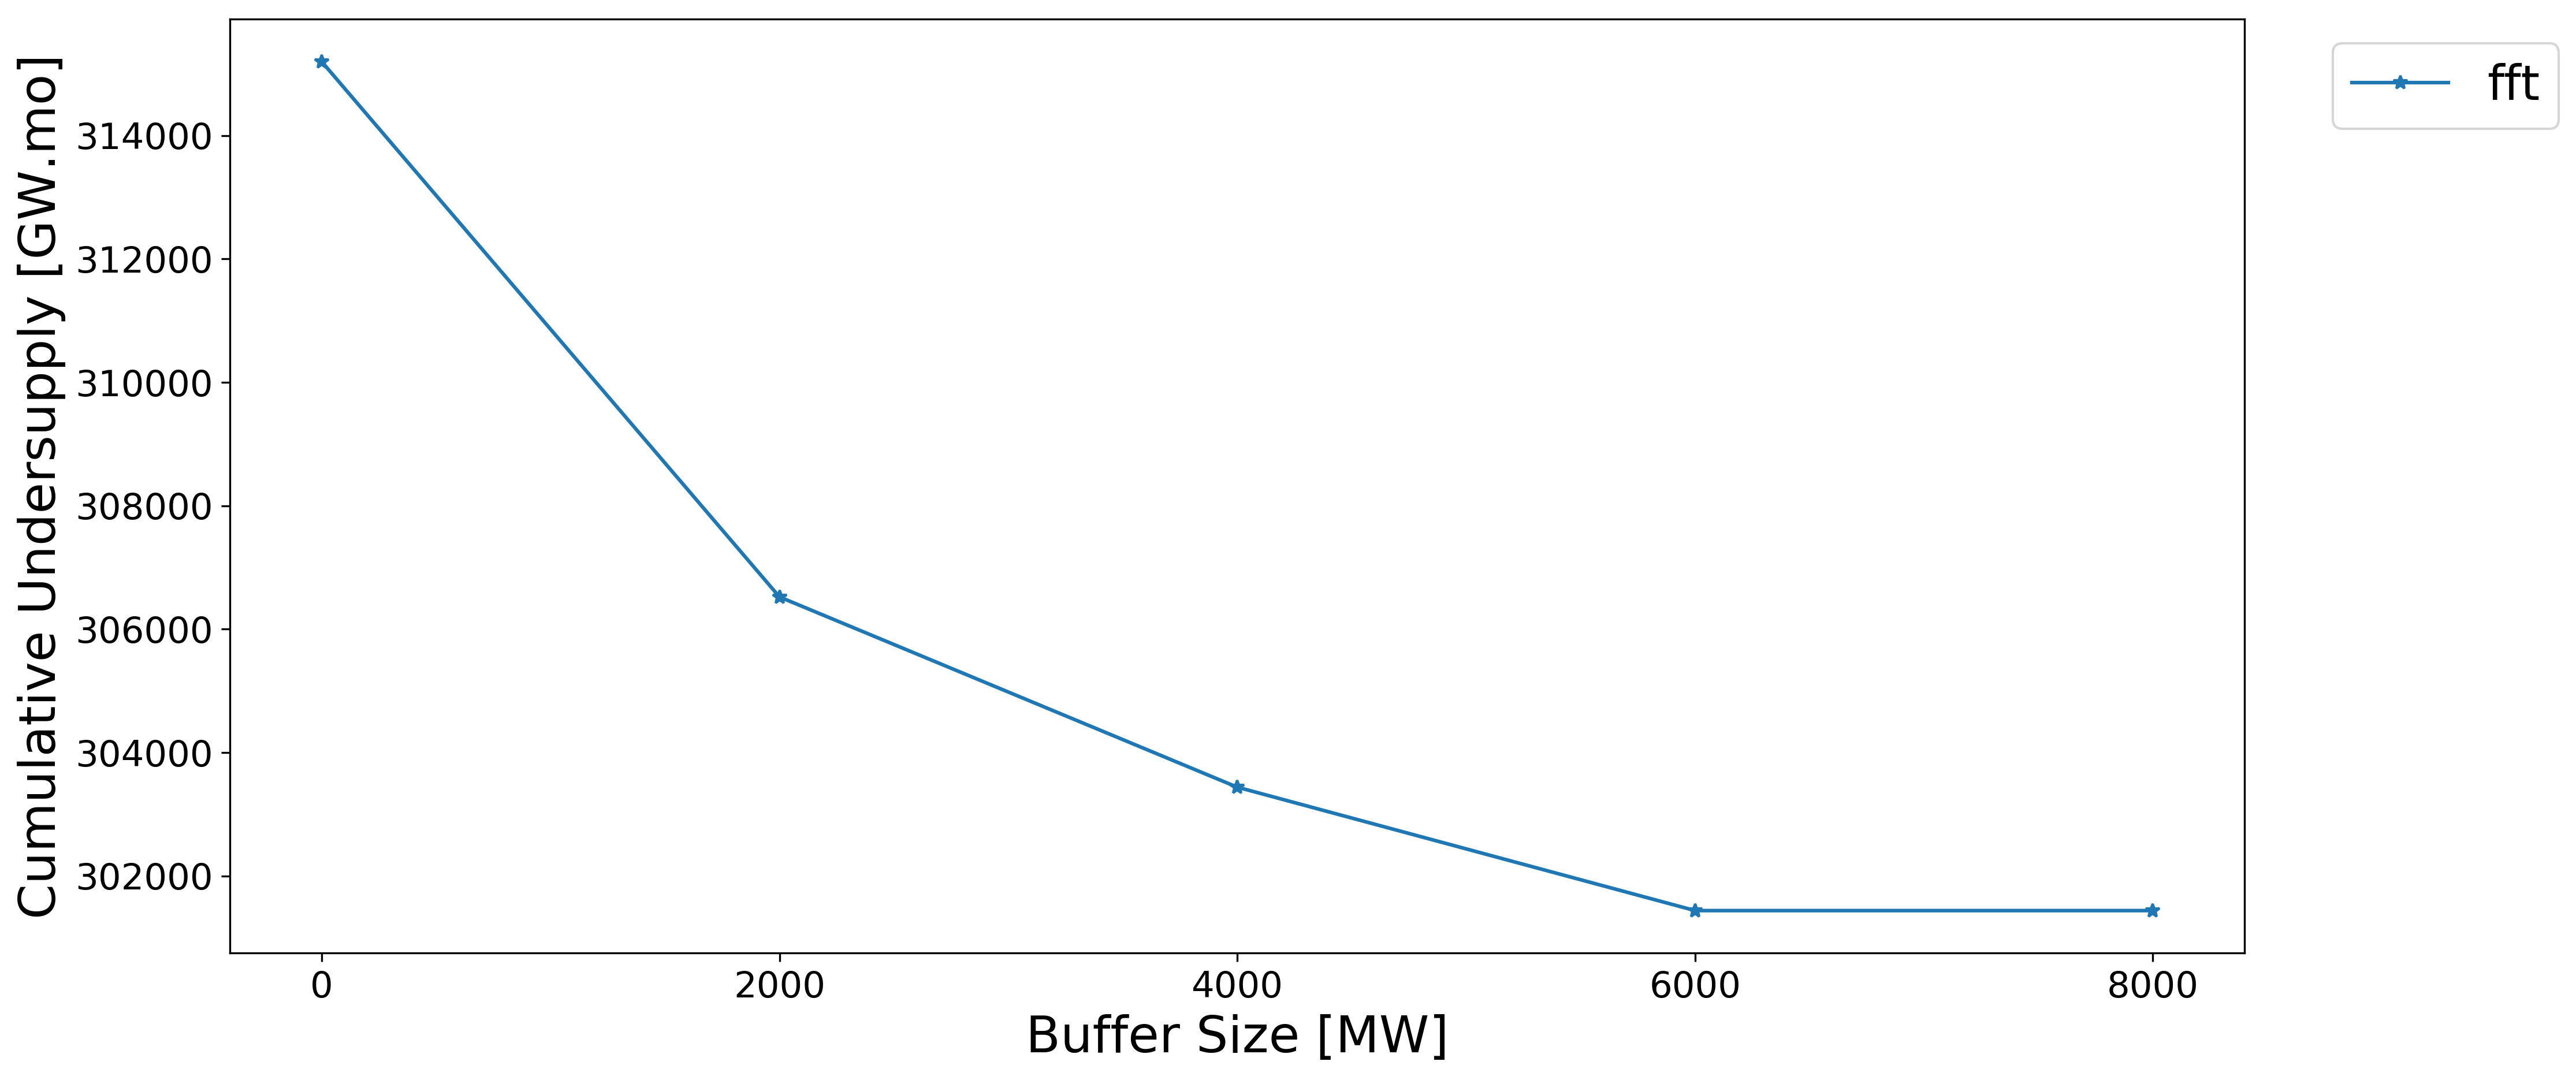
\includegraphics[width=\linewidth]{24-sens-buffer.png} 
		\caption{Under Supply}
		\label{fig:23undersupply}
	\end{subfigure}
	\vspace{1cm}
	\begin{subfigure}[t]{0.8\textwidth}
		\centering
		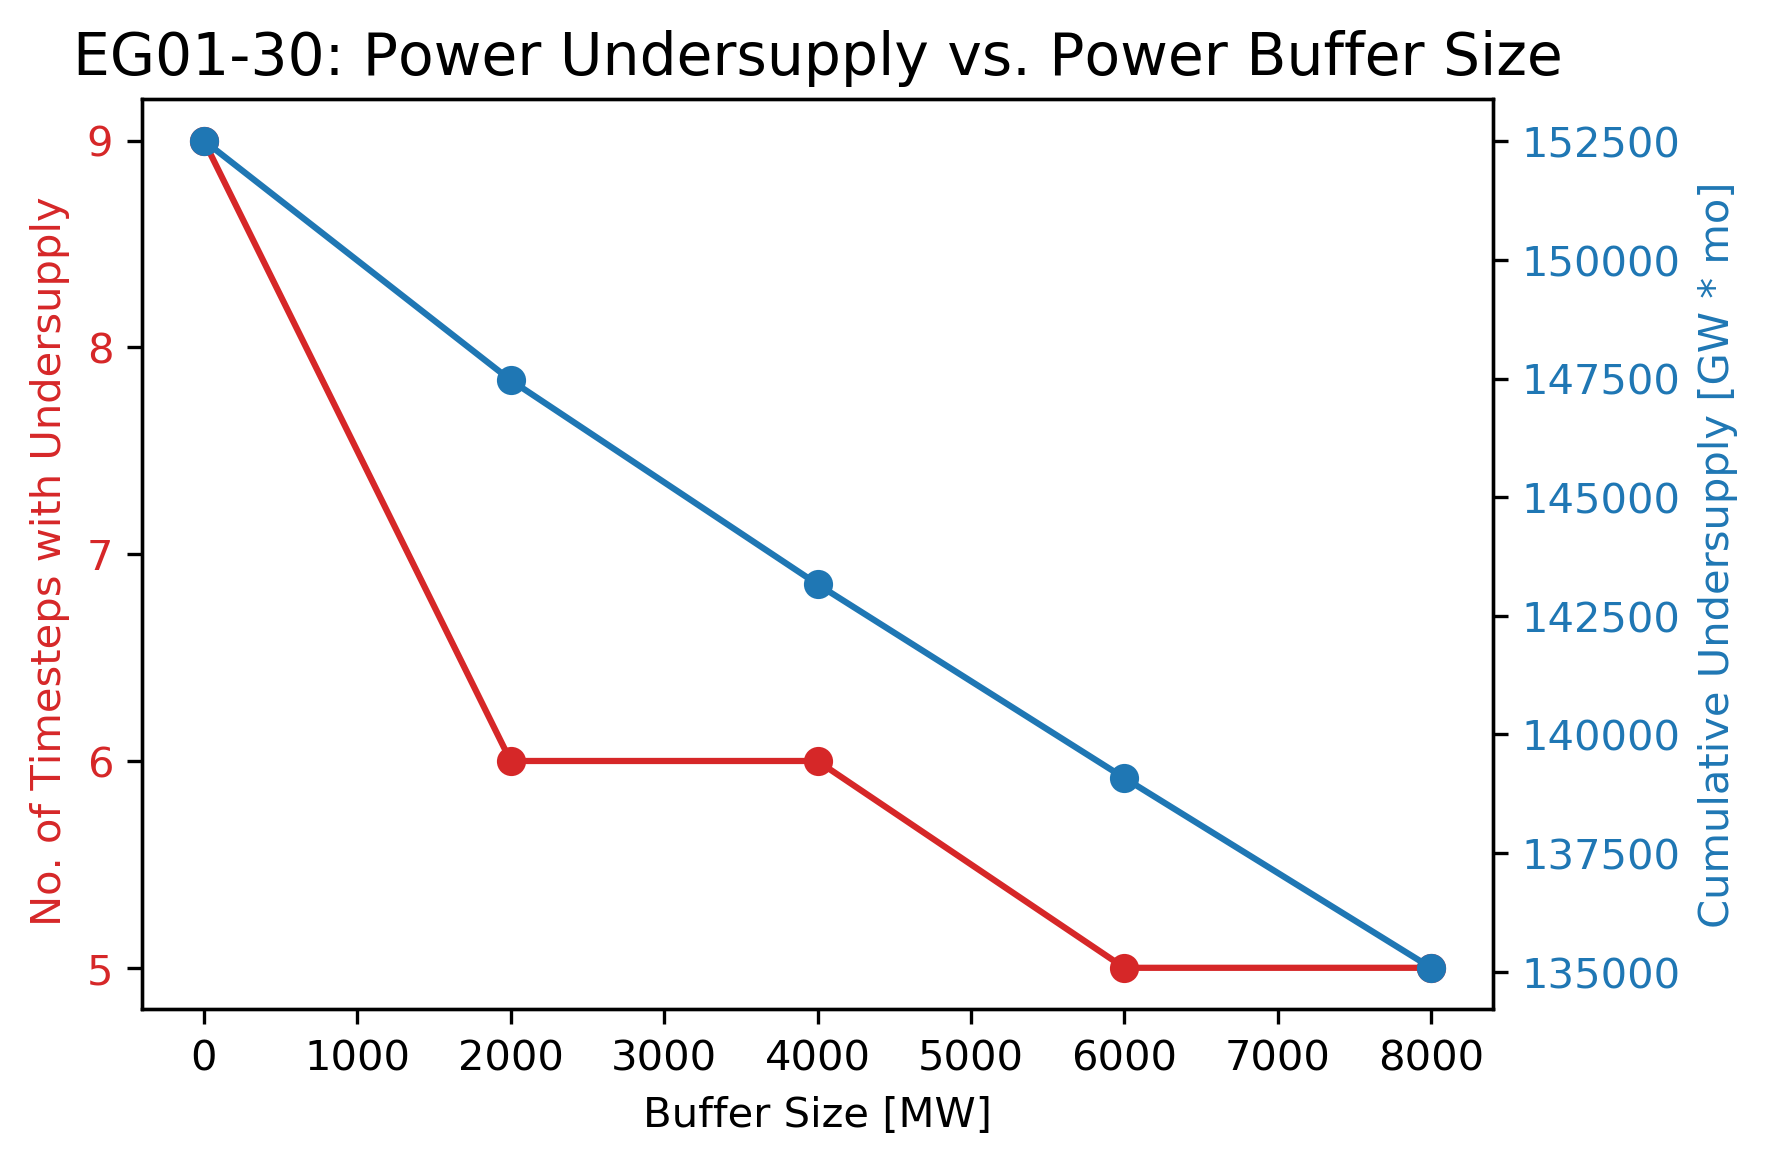
\includegraphics[width=\linewidth]{30-sens-buffer.png} 
		\caption{Under Capacity}
		\label{fig:23undercapacity}
	\end{subfigure}
	\hfill
	\caption{Comparison of undersupply}
	\label{fig:sabuffer}
\end{figure}

\begin{table}[h]
	\centering
	\caption{Dependency of the undersupply of Power on the buffer size.}
	\label{tab:buff_size}
	\footnotesize
		\begin{tabularx}{\textwidth}{RRRRR}
                \hline
        Buffer [MW]     &      & EG01-24   & EG01-30 \\
		\hline
		0             & Undersupplied $[\#]$ & 20 & 9\\  
                      & Cumulative $[GW]$    & 315917 & 152517 \\ \hline
        2000          & Undersupplied $[\#]$ & 9 & 6 \\  
        	      & Cumulative $[GW]$    & 306520 & 147166 \\ \hline
        4000          & Undersupplied $[\#]$ & 8 & 6 \\  
				  & Cumulative $[GW]$    & 303438 & 143166 \\ \hline
		6000          & Undersupplied $[\#]$ & 7 & 5 \\  
		& Cumulative $[GW]$    & 303438 & 139083 \\ \hline
        8000          & Undersupplied $[\#]$ & 7 & 5  \\  
	              & Cumulative $[GW]$    & 303438 & 135083 \\ \hline
	\end{tabularx}
\end{table}

\subsection{Best Performance Models}
Table %\ref{tab:bestinputs} 
shows \deploy input parameters for
EG01-EG23, EG01-EG24, EG01-EG29, and EG01-EG30 transition scenarios
that minimizes undersupply of power and minimizes 
the undersupply and under capacity of the other facilities. 
The need for buffers for commodities is a reflection of reality
in which ideally a supply cushion exists to ensure that there 
is available supply in the case of unexpected undersupply. 

Figure \ref{fig:}

\begin{figure}[]
	\centering
	\begin{subfigure}[t]{1.2\textwidth}
		\centering
		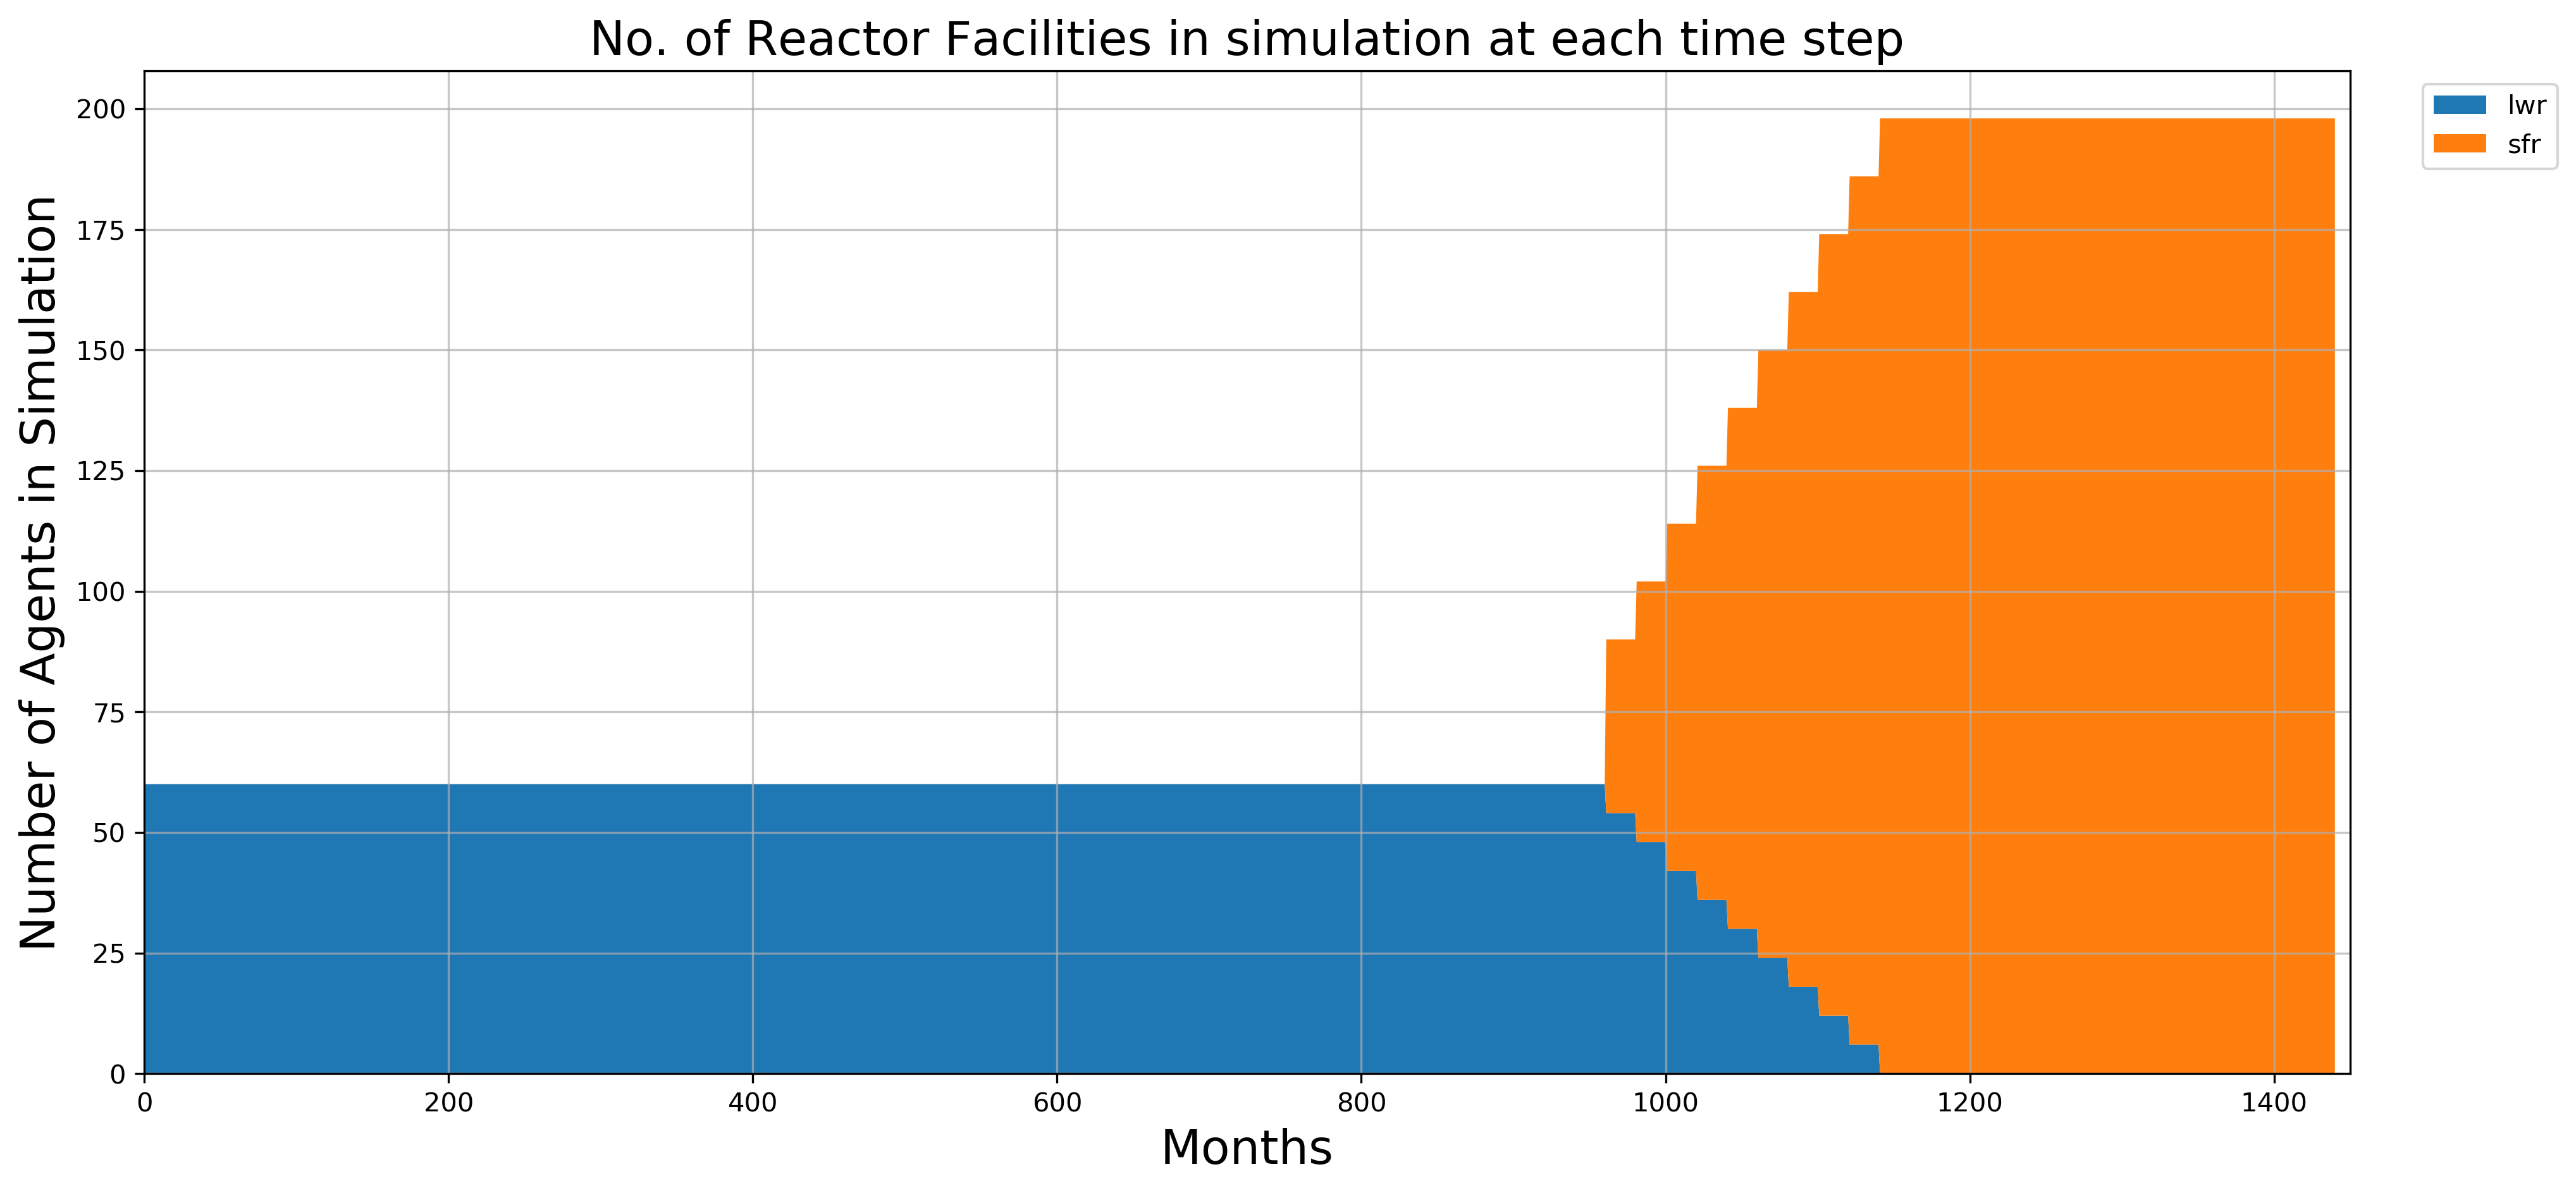
\includegraphics[width=\linewidth]{eg23-stack_reactor.png} 
		\caption{EG01-23: Reactor Deployment}
		\label{fig:23reactor}
	\end{subfigure}
	\vspace{1cm}
	\begin{subfigure}[t]{1.2\textwidth}
		\centering
		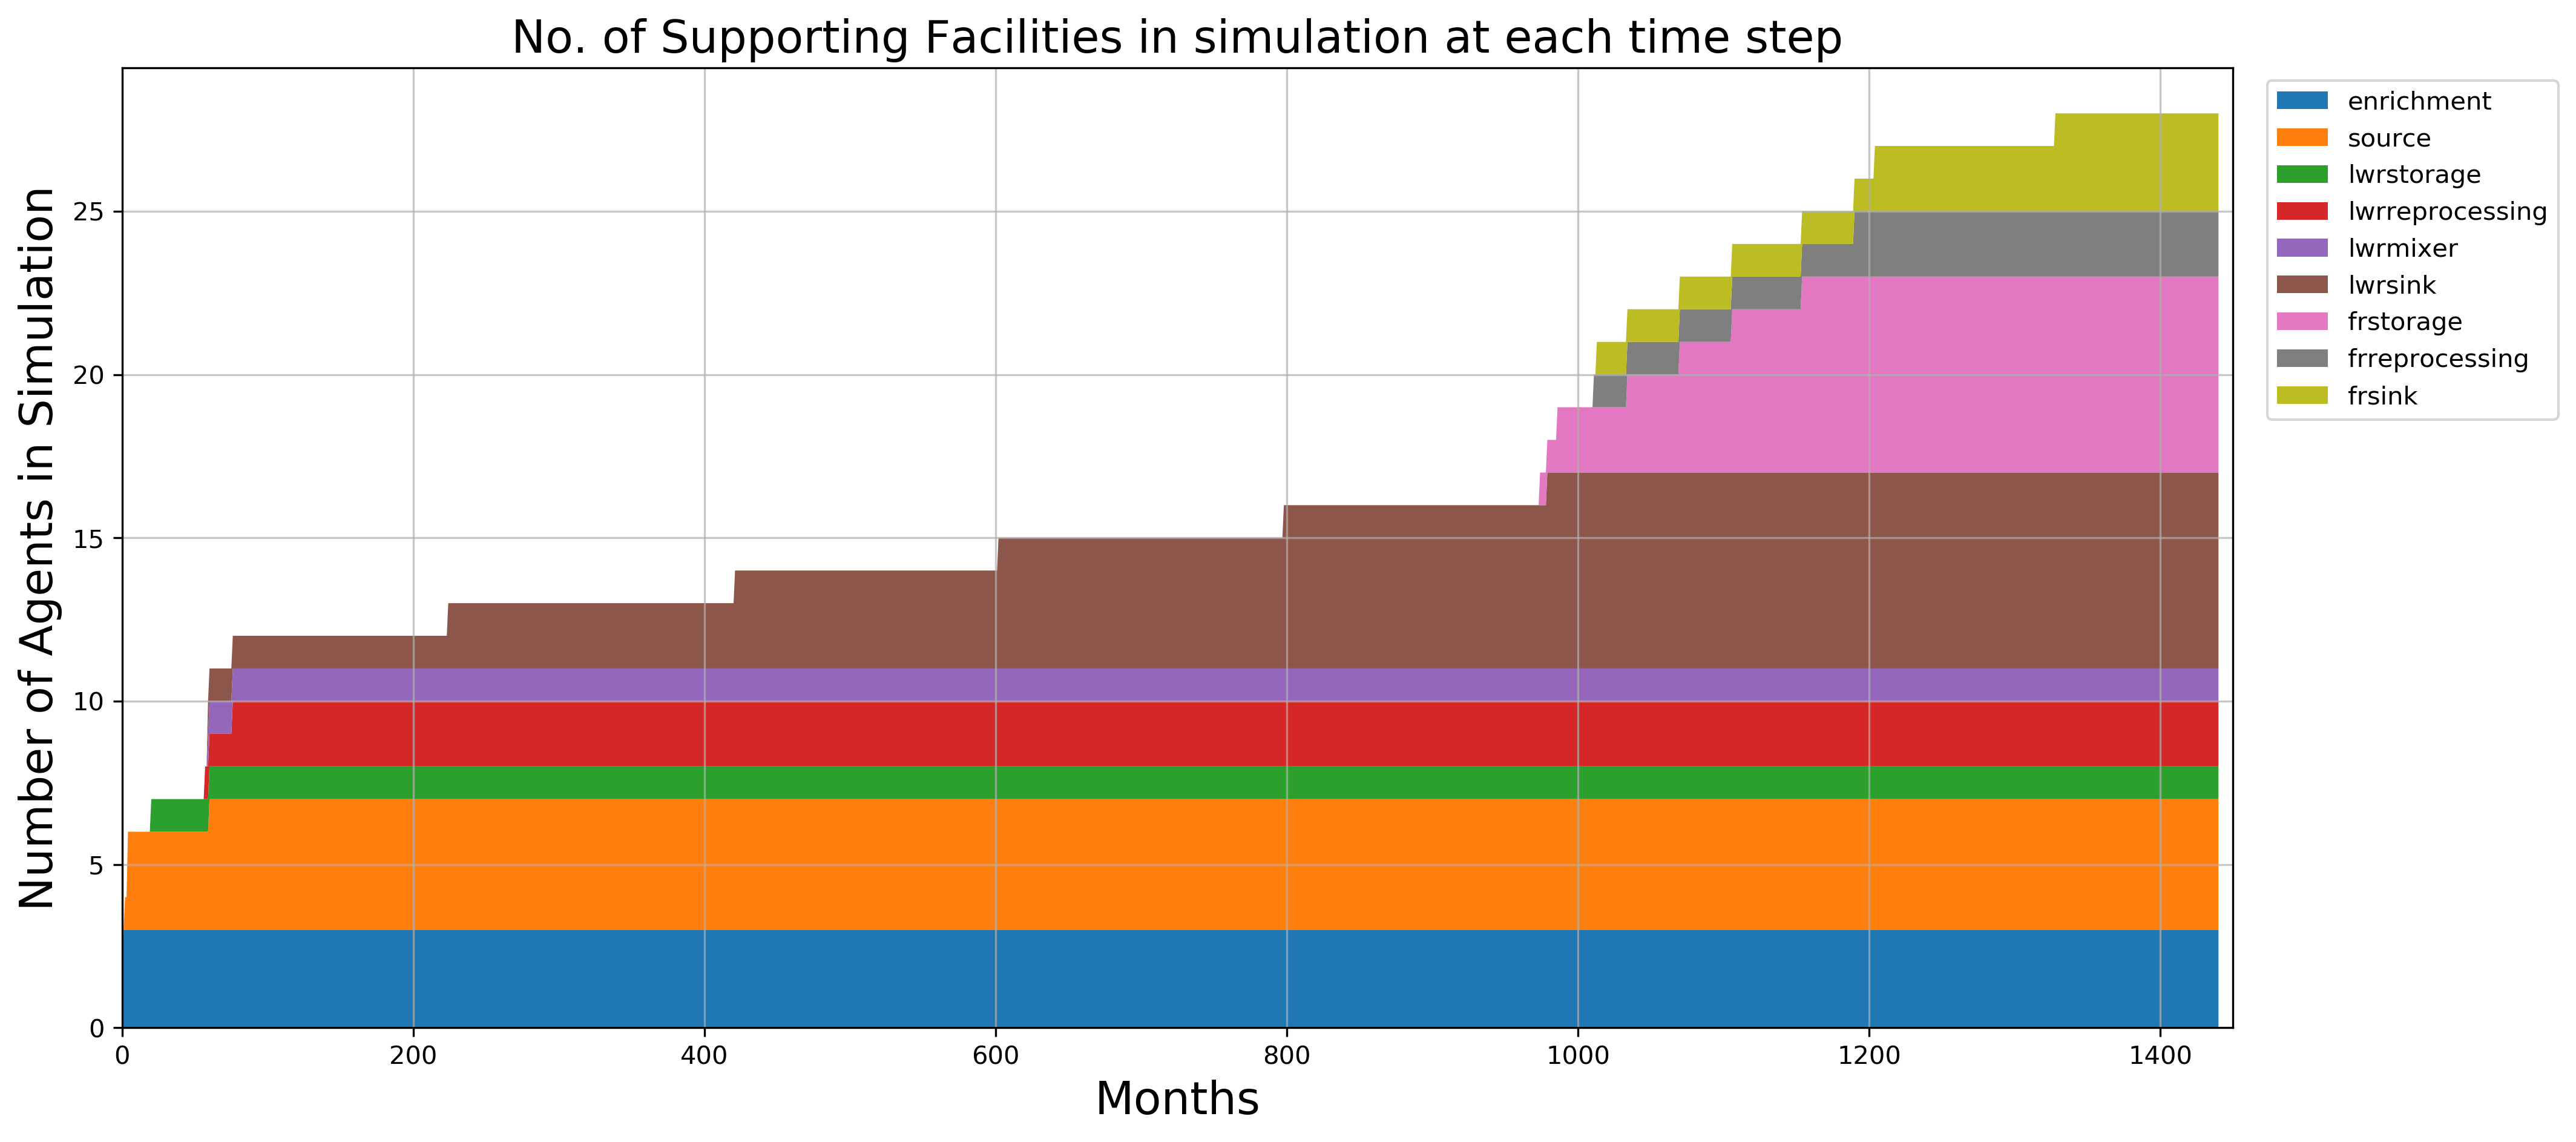
\includegraphics[width=\linewidth]{eg23-stack_support.png} 
		\caption{EG01-23: Supporting Facility Deployment}
		\label{fig:23support}
	\end{subfigure}
	\hfill
	\caption{Time dependent deployment of reactor and supporting facilities in 
	the EG01-23 constant power demand transition scenario. 
	\deploy automatically deploys reactor and supporting facilities 
	to set up a supply chain to meet constant power demand of 60000MW 
	during a transition from \glspl{LWR} to \glspl{SFR}. }
	\label{fig:23stack}
\end{figure}

\begin{figure}[]
	\centering
	\begin{subfigure}[t]{1.2\textwidth}
		\centering
		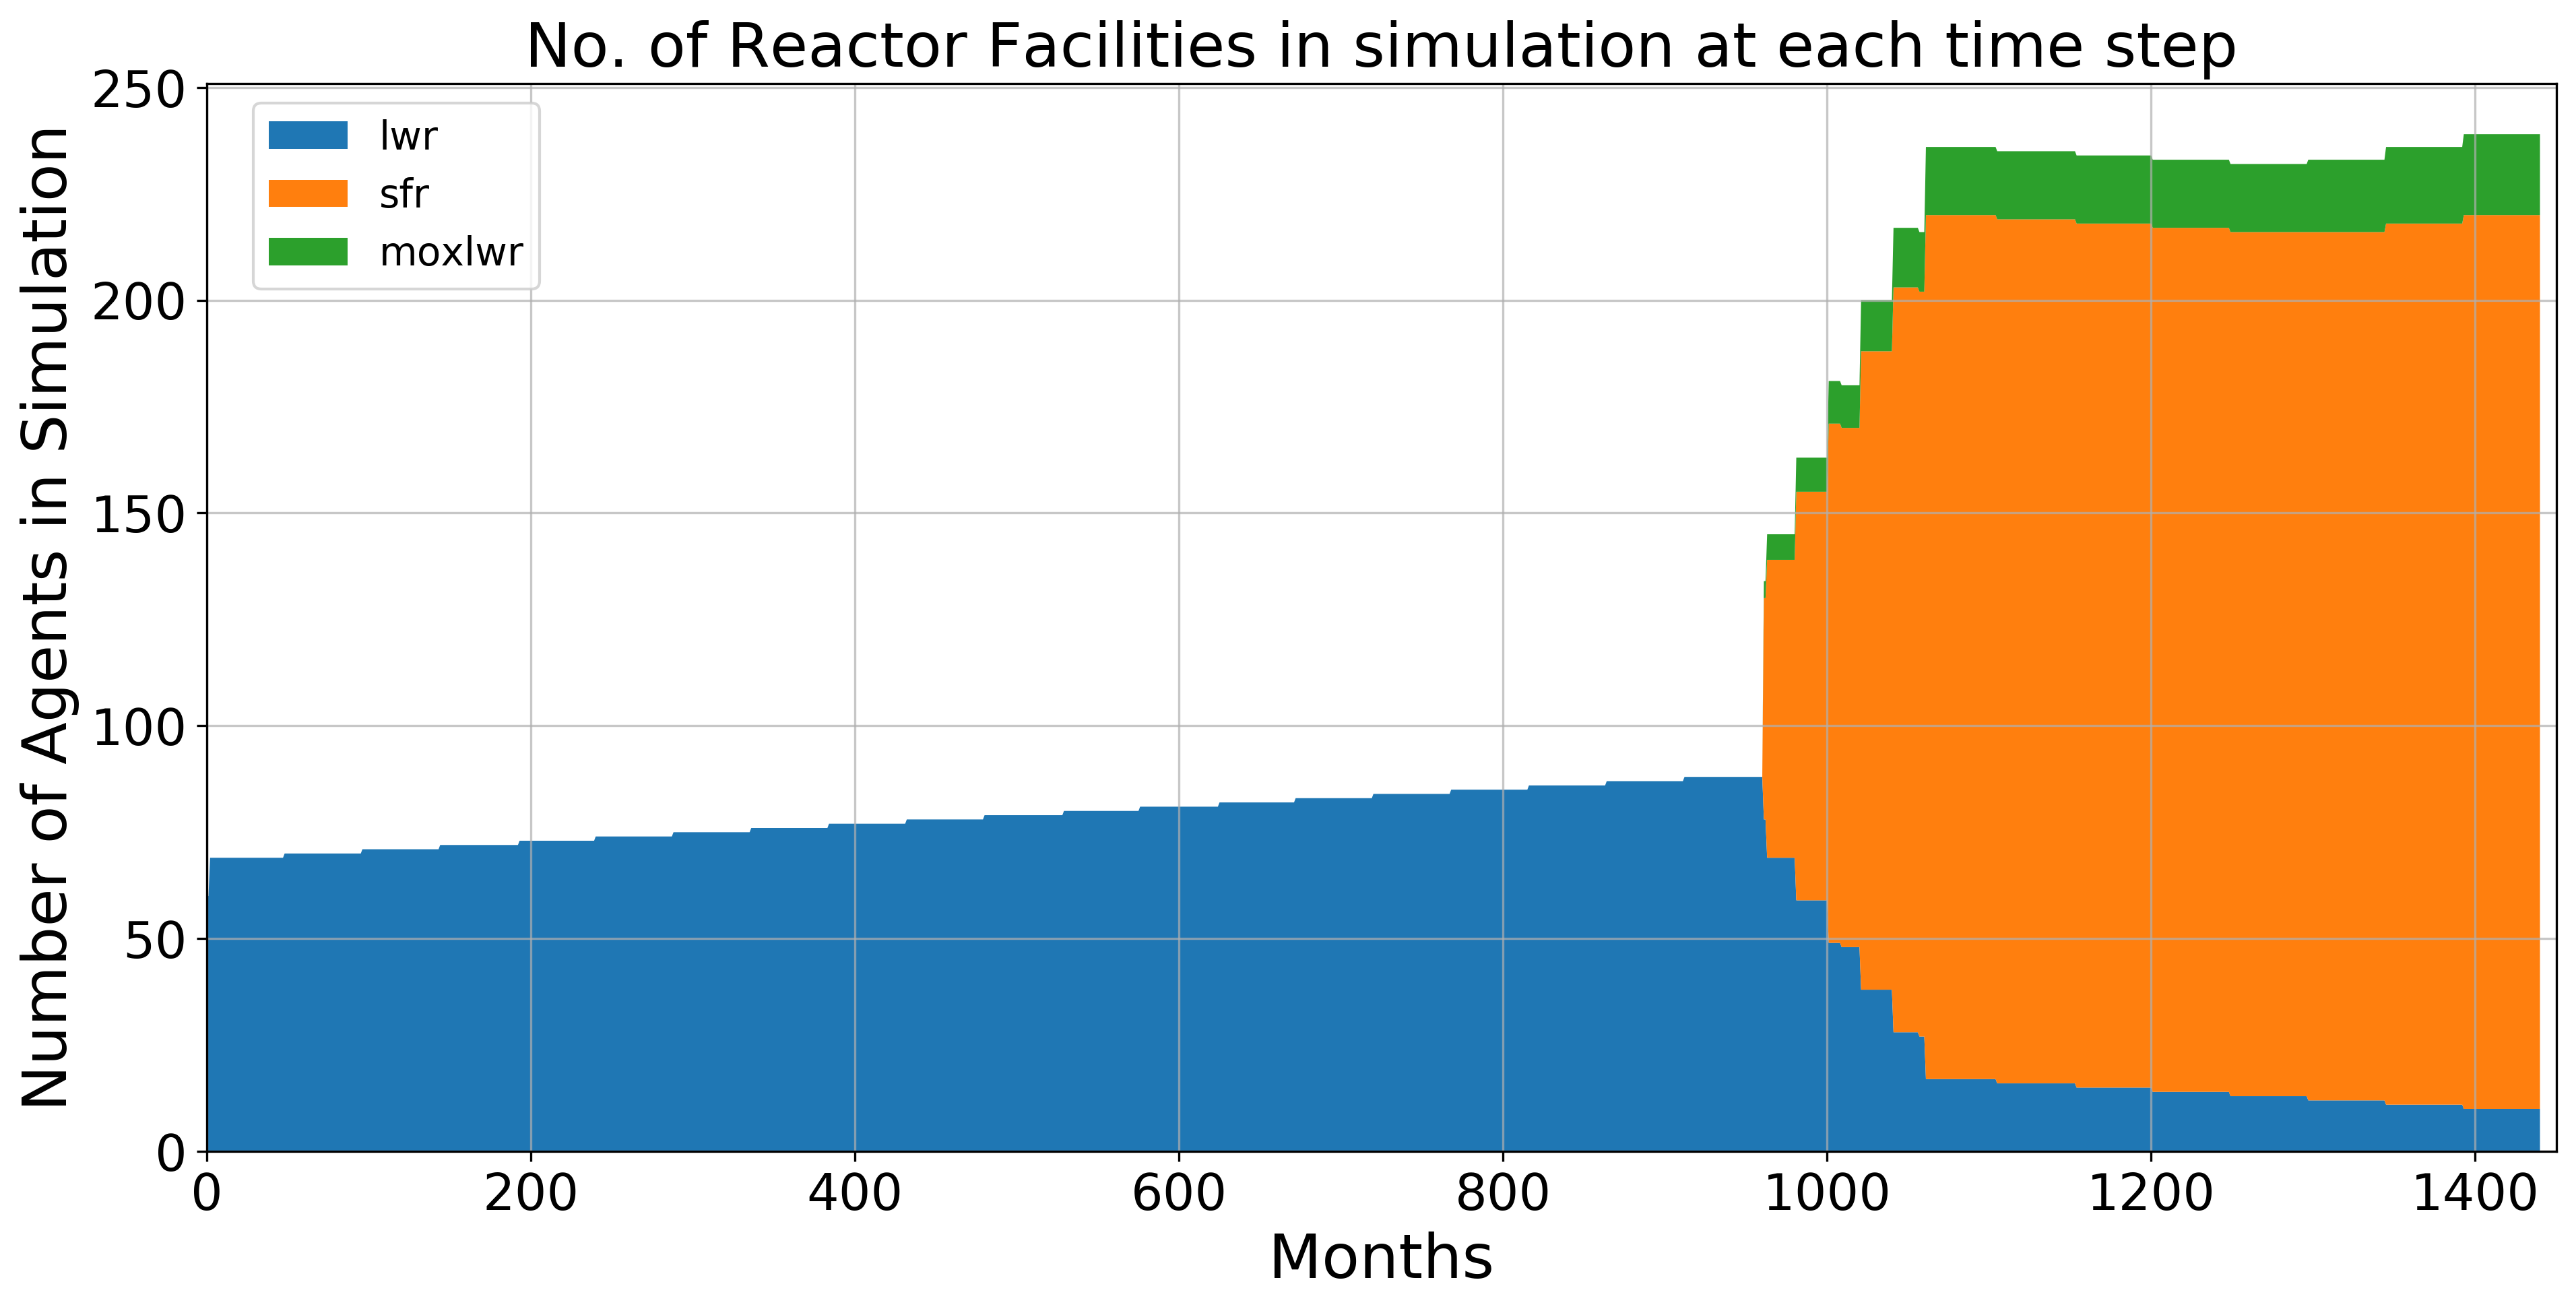
\includegraphics[width=\linewidth]{eg30-stack_reactor.png} 
		\caption{EG01-30: Reactor Deployment}
		\label{fig:30reactor}
	\end{subfigure}
	\vspace{1cm}
	\begin{subfigure}[t]{1.2\textwidth}
		\centering
		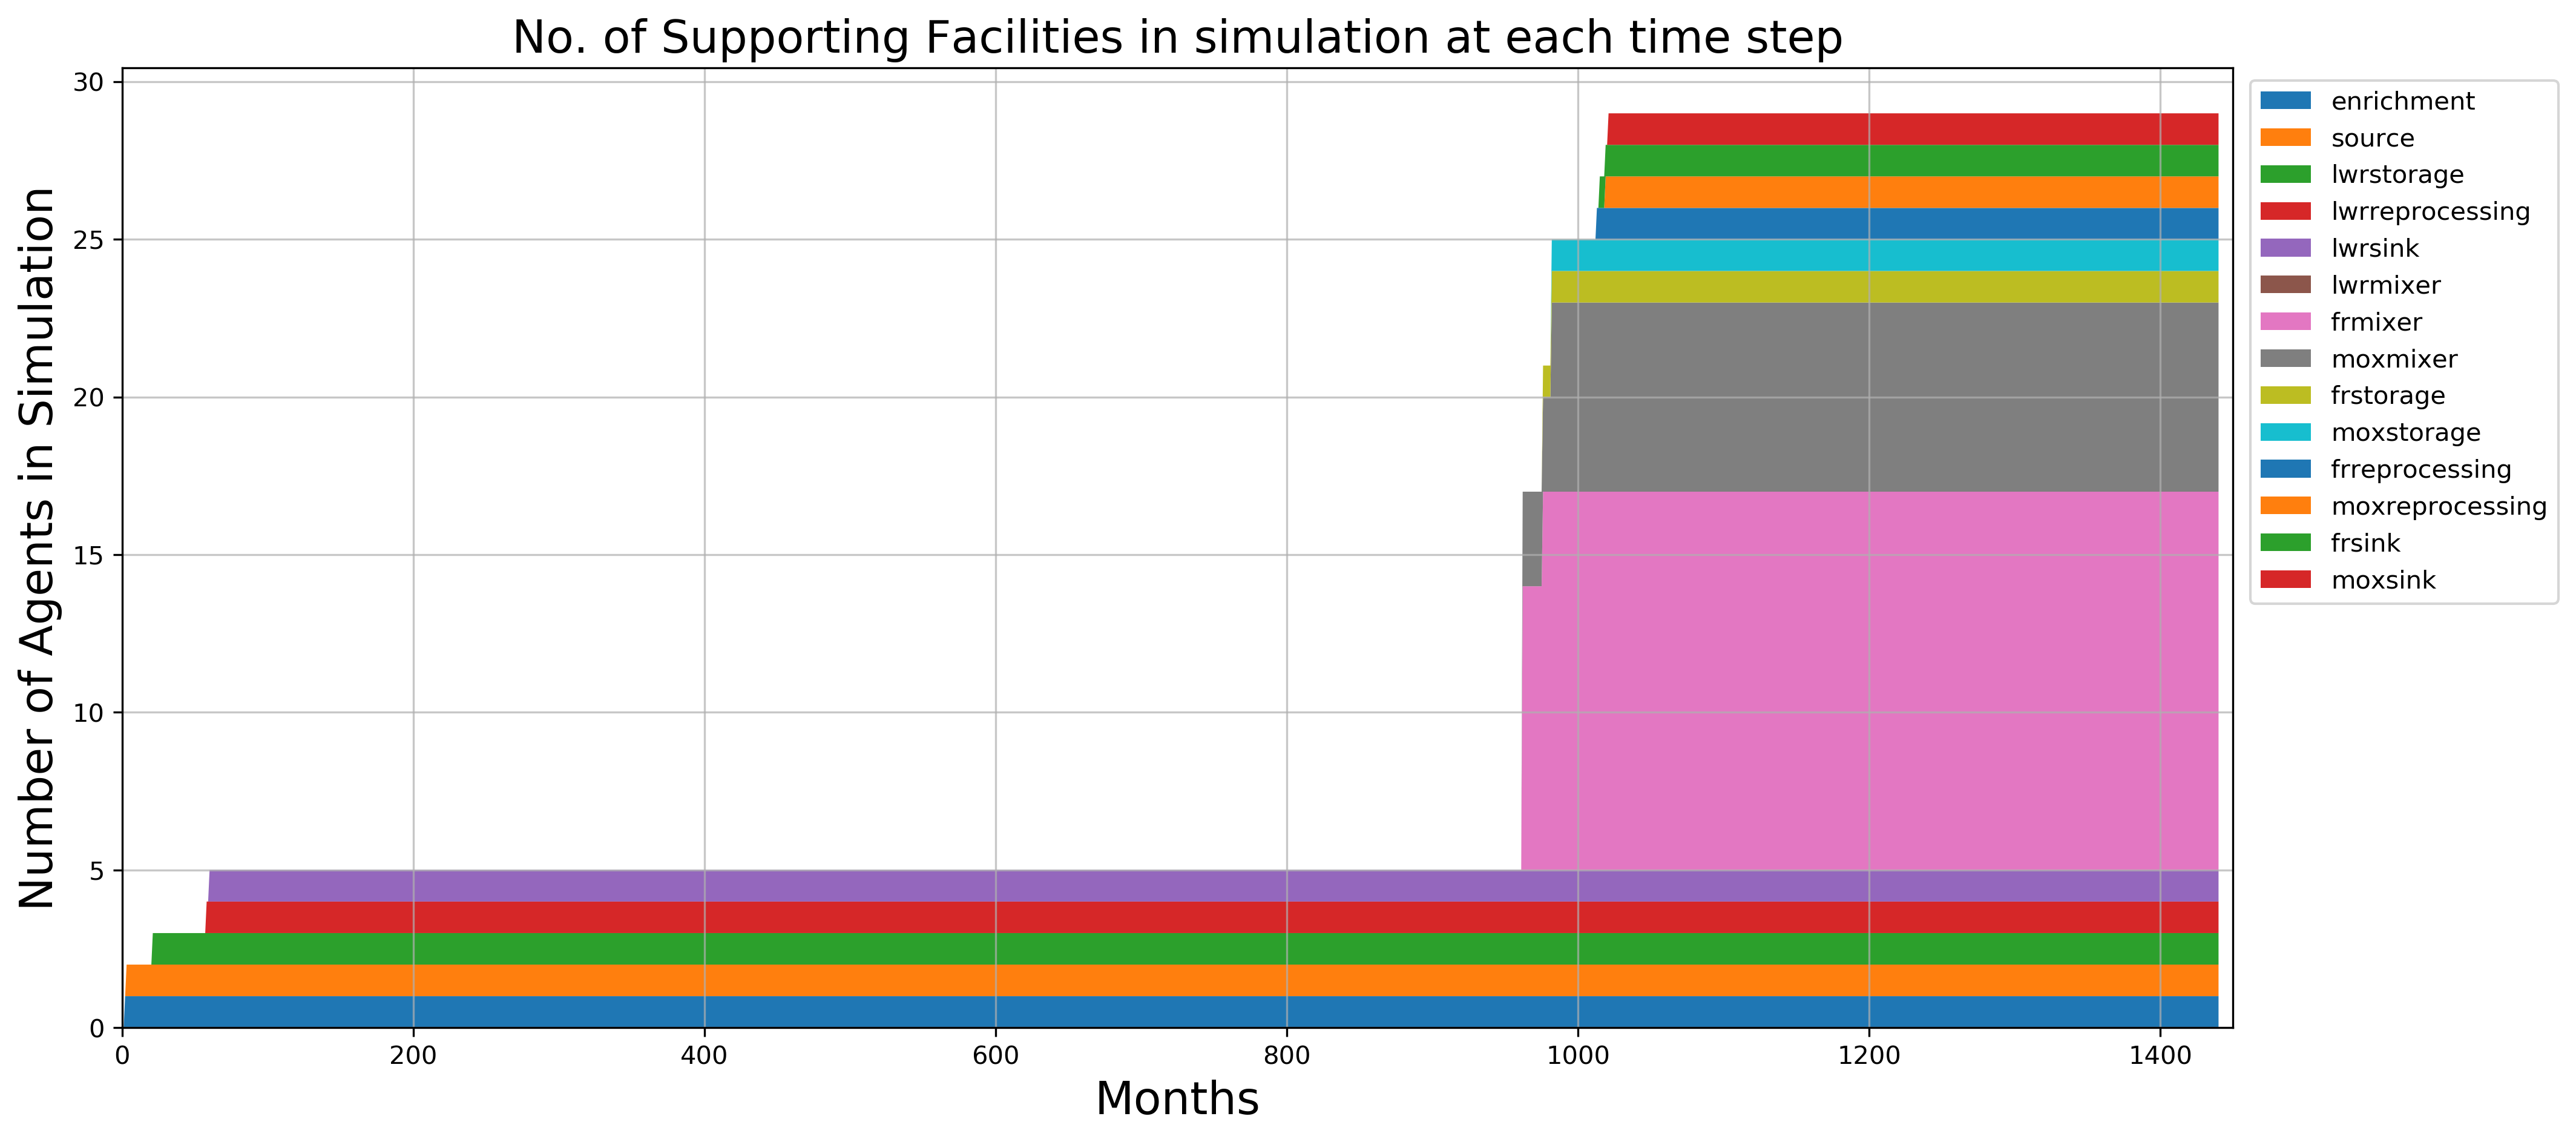
\includegraphics[width=\linewidth]{eg30-stack_support.png} 
		\caption{EG01-30: Supporting Facility Deployment}
		\label{fig:30support}
	\end{subfigure}
	\hfill
	\caption{Time dependent deployment of reactor and supporting facilities in 
	the EG01-30 linearly increasing power demand transition scenario. 
	\deploy automatically deploys reactor and supporting facilities 
	to set up a supply chain to meet constant power demand of $60000 + 250*t/12$ MW
	during a transition from \glspl{LWR} to MOX LWRs and \glspl{SFR}. }
	\label{fig:23stack}
\end{figure}

%INSERT TABLE \ref{tab:undersupply}%